\begin{frame}[allowframebreaks]{Relative Position of Image Patches}
    \begin{figure}
        \centering
        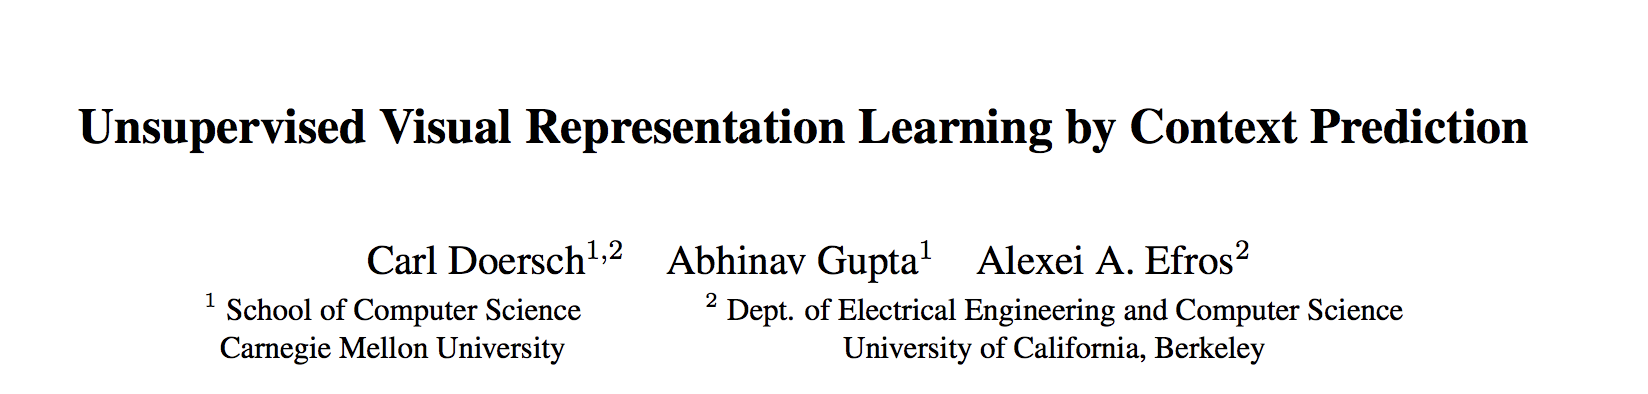
\includegraphics[width=1\linewidth,height=\textheight,keepaspectratio]{images/ssl/slide_29_2_img.png}
    \end{figure}
    \begin{figure}
        \centering
        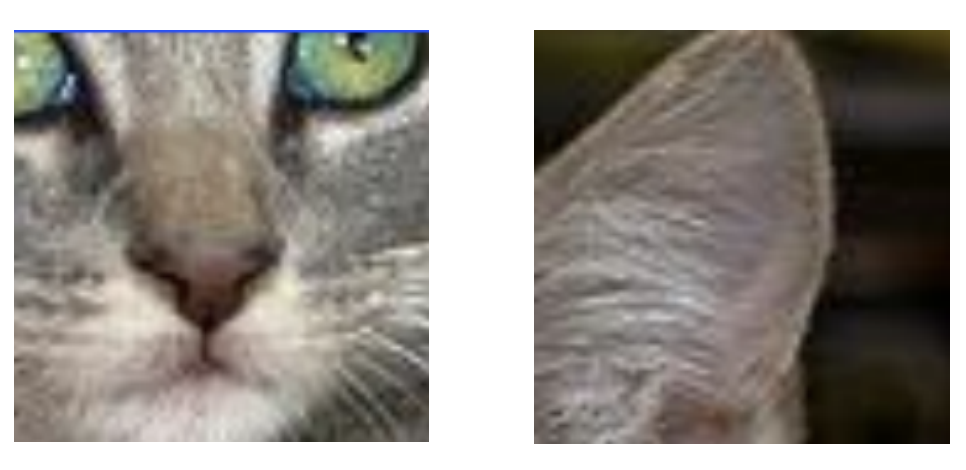
\includegraphics[width=0.5\linewidth,height=0.6\textheight,keepaspectratio]{images/ssl/slide_29_1_img.png}
        
        Slide: Zisserman et al (2019). Relative Position of Image Patches.
    \end{figure}

    \textbf{Task}: Predict the relative position of the second patch with respect to the first


    \framebreak

    \textbf{Shuffle image patches; predict their relative spatial positions.}
    \begin{itemize}
        \item The input image is divided into several non-overlapping patches.
        \item These patches are randomly shuffled to disrupt their original spatial arrangement.
        \item The model is tasked with predicting the original relative positions of the shuffled patches.
    \end{itemize}

    \framebreak

    \begin{figure}
        \centering
        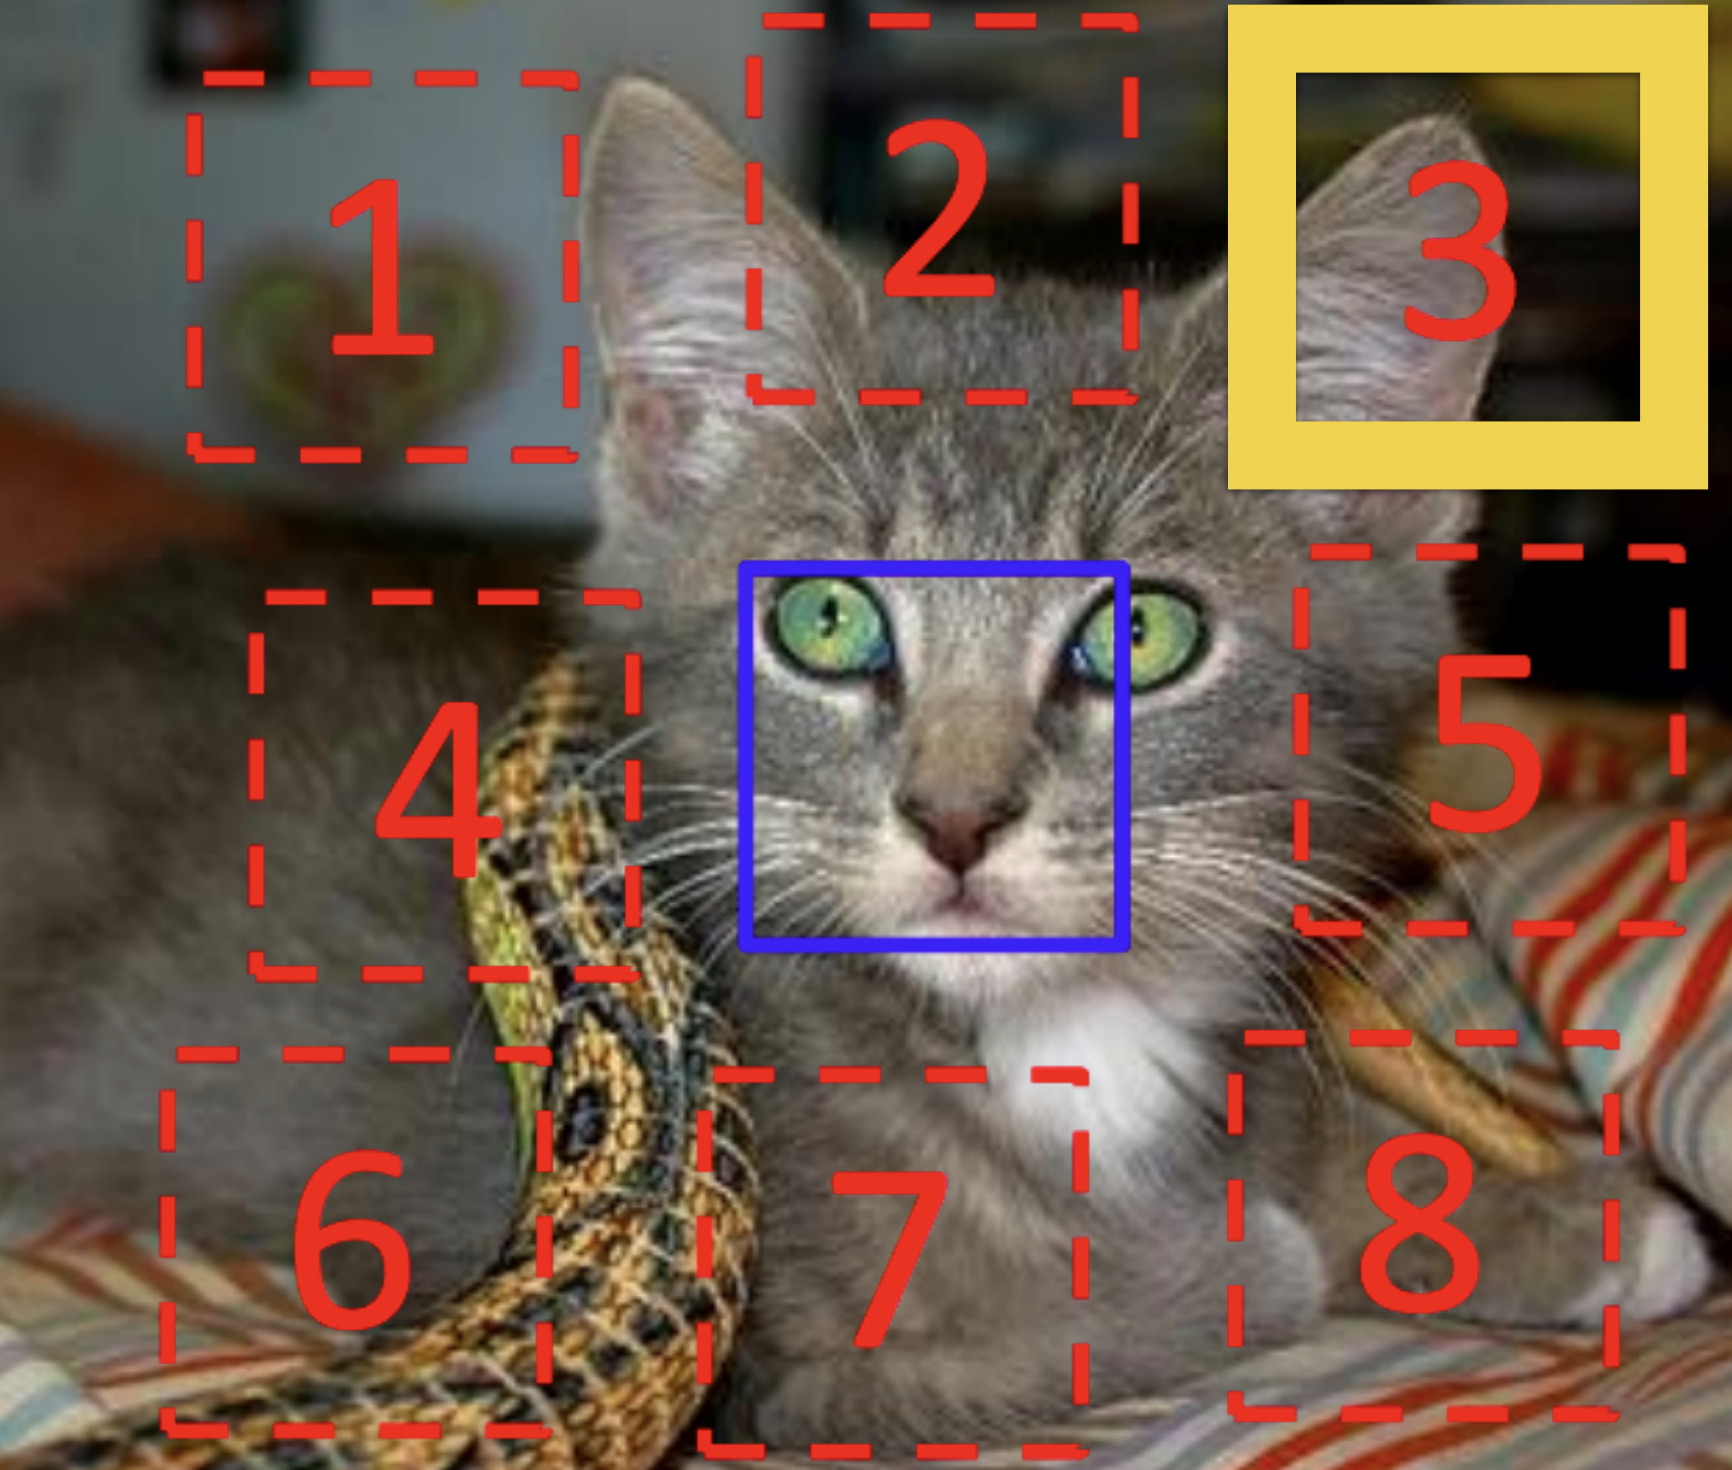
\includegraphics[width=\linewidth,height=0.9\textheight,keepaspectratio]{images/ssl/slide_30_1_img.png}
    \end{figure}

    \framebreak

    \begin{figure}
        \centering
        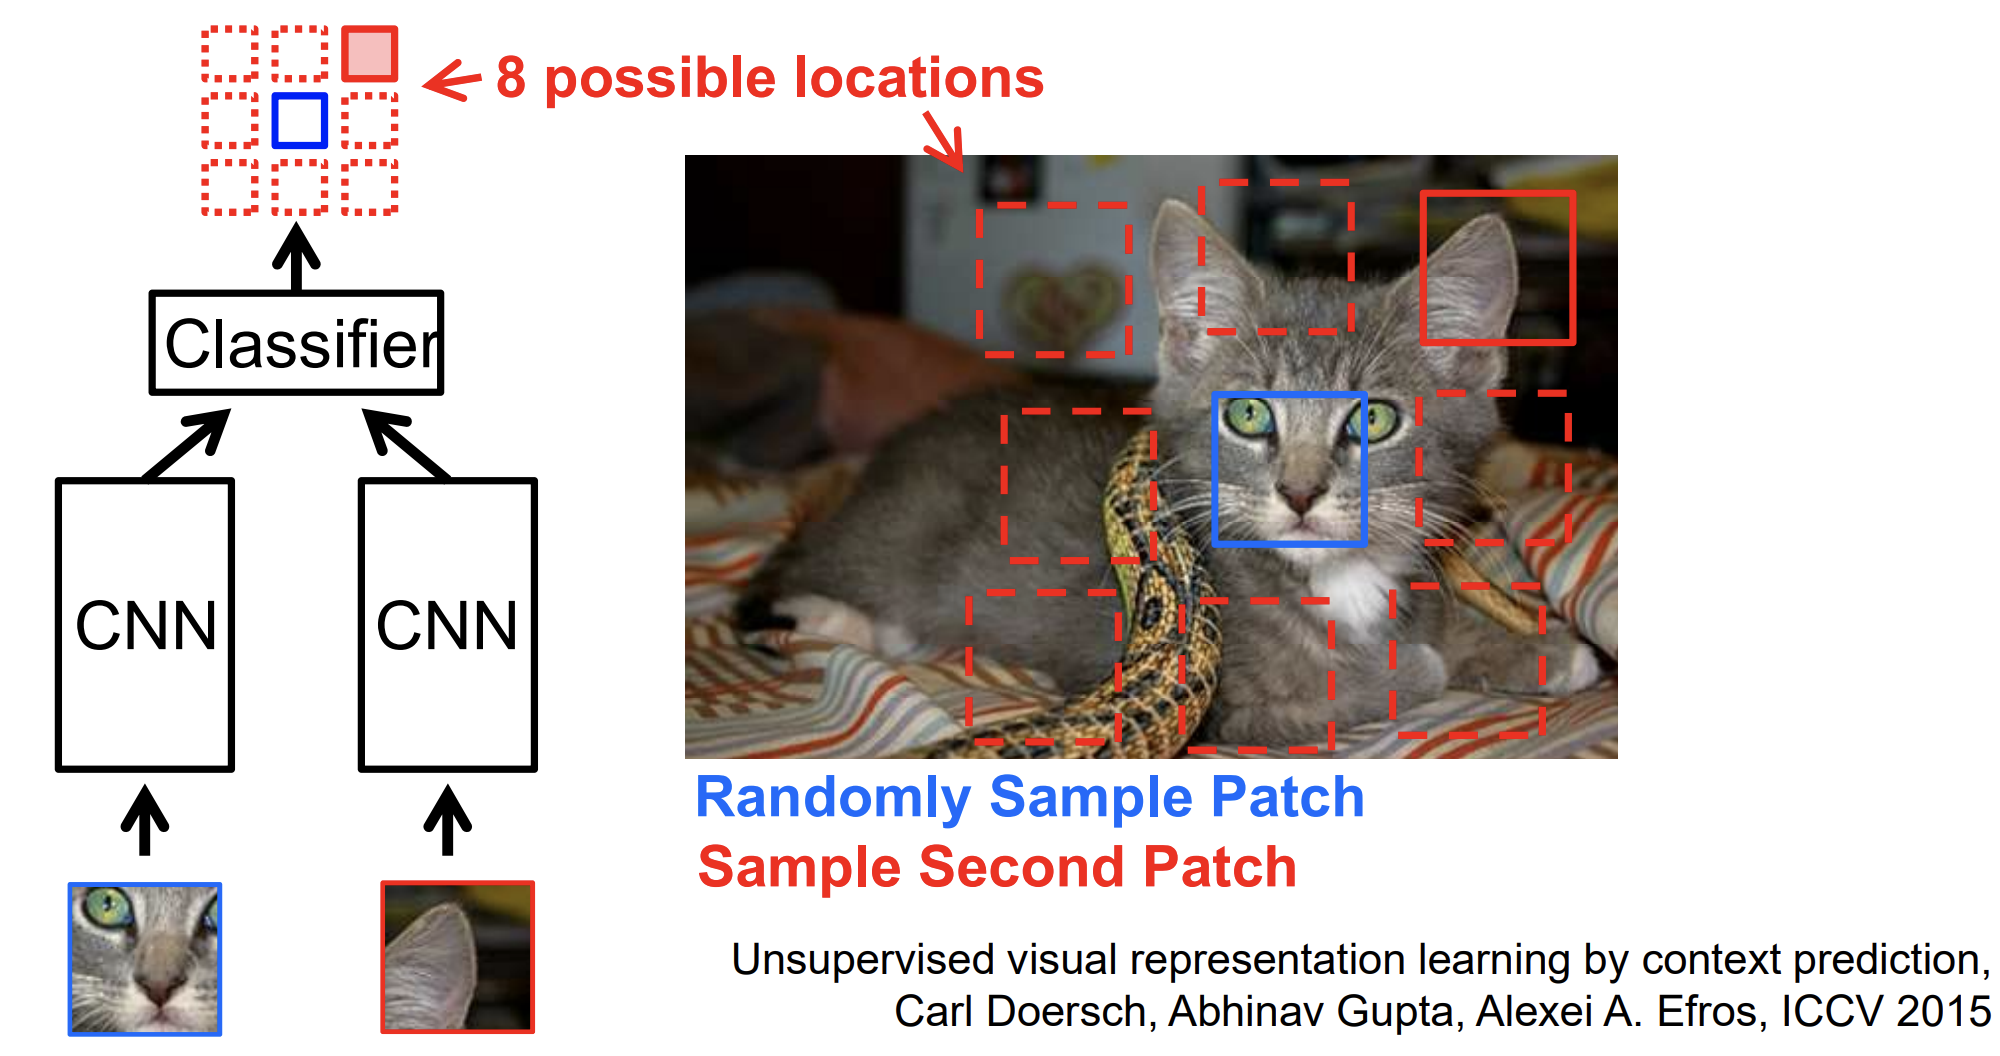
\includegraphics[width=\linewidth,height=0.9\textheight,keepaspectratio]{images/ssl/slide_31_1_img.png}
    \end{figure}

    \framebreak

    \textbf{Model learns geometric relationships and spatial context.}
    \begin{itemize}
        \item By solving the patch position prediction task, the model is forced to understand the underlying spatial structure of objects and scenes.
        \item This encourages the learning of features that capture geometric relationships between different parts of the image.
        \item Such self-supervised tasks help the model develop a strong sense of spatial context, which is beneficial for downstream vision tasks like object detection and segmentation.
    \end{itemize}

    \framebreak

    \textbf{Solving Jigsaw puzzles as a pretext task.}

    \begin{figure}
        \centering
        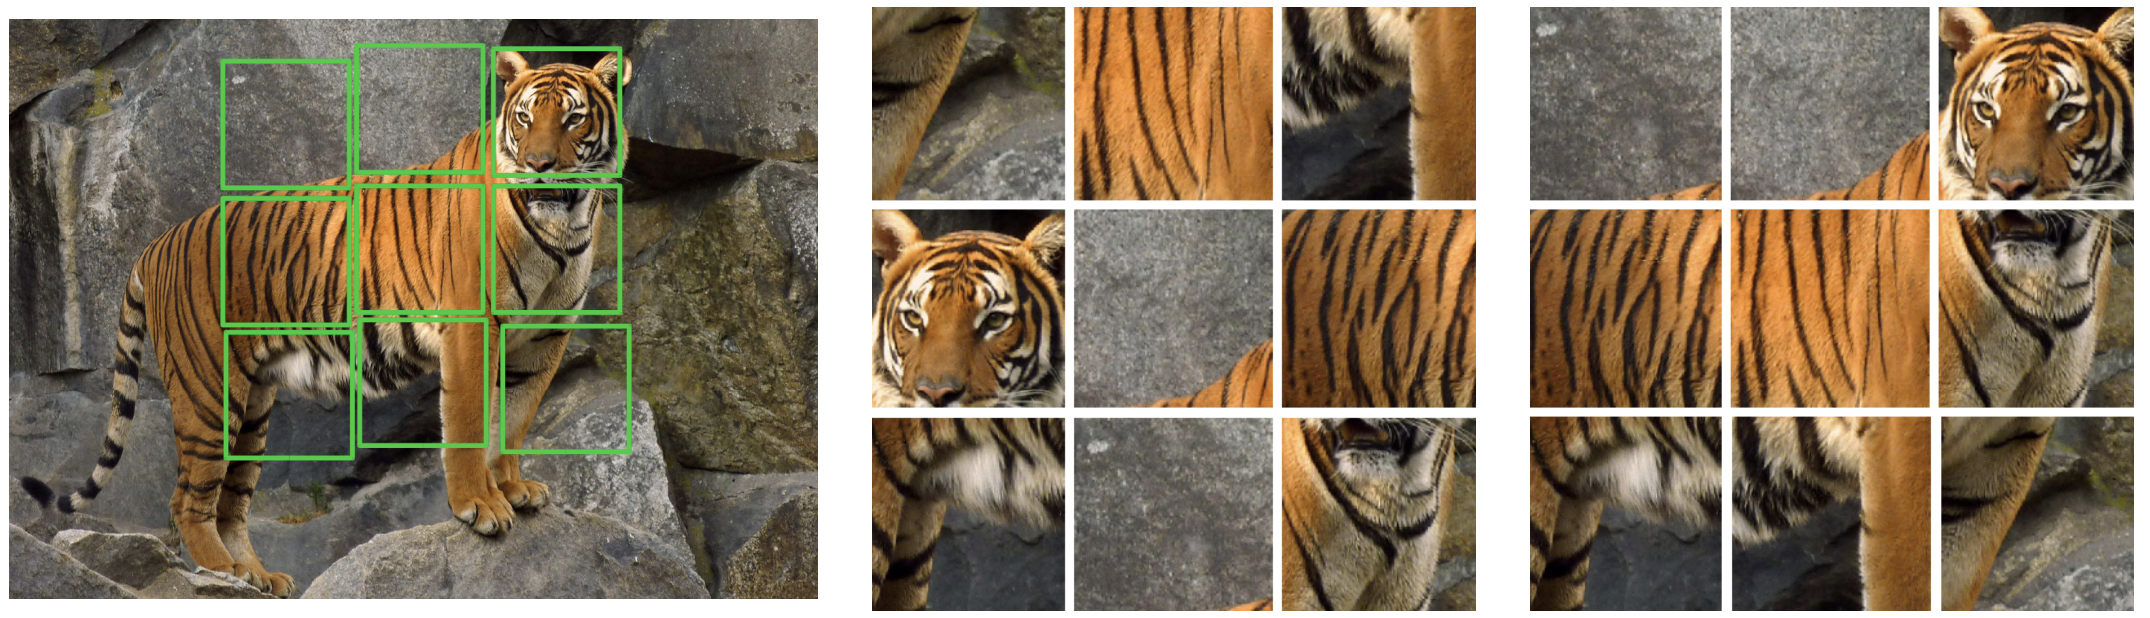
\includegraphics[width=\linewidth,height=0.9\textheight,keepaspectratio]{images/ssl/slide_32_1_img.png}
    \end{figure}
\end{frame}